\documentclass{beamer}
\usetheme{metropolis} % Use metropolis theme


\title{ECON 3818: Introduction to Statistics with Computer Applications}
%\subtitle
\date{\today}
\author{Kyle Butts}

\definecolor{blue}{RGB}{0,114,178}
\definecolor{red}{HTML}{EB0E09}
\definecolor{yellow}{RGB}{240,228,66}
\definecolor{green}{RGB}{0,158,115}
\definecolor{maroon}{HTML}{AF3335}
\definecolor{purple}{HTML}{7E90B8}

\definecolor{mybackground}{HTML}{ECECEC}
\setbeamercolor{background canvas}{bg= mybackground}

\definecolor{buff-gold}{HTML}{CFB87C}
\definecolor{buff-grey}{HTML}{565A5C}
\definecolor{buff-lightgrey}{HTML}{A2A4A3}
\definecolor{buff-black}{HTML}{000000}

\setbeamercolor{alerted text}{fg=buff-gold!80!black}
\setbeamercolor{frametitle}{bg=buff-black}
\setbeamercolor{title}{fg=buff-grey}
\setbeamercolor{button}{bg=buff-gold}

% Allow to remove indent w/ \begin{itemize}[leftmargin= *]
\usepackage{enumitem}
\setlist[itemize]{label= \textbullet}

% \usepackage[libertine]{newtxmath}
\usepackage{longtable}
\usepackage{booktabs}
\usepackage{enumitem}

\begin{document}

% Title Page ---------------------------------------
\maketitle

% Expectations -------------------------------------
\section{Expectations}

\begin{frame}{Outline}
	
	\alert{Expectation}
	\begin{itemize}
		\item Definition
		\item Properties
	\end{itemize}
		
	\alert{Variance}
	\begin{itemize}
		\item Definiton
		\item Properties
		      
	\end{itemize}
	
\end{frame}

\begin{frame}{What are Expectations?}
	We are familiar with expectations. For example, 
	\begin{itemize}
		\item What salary can I expect to earn after graduating from college?
		\item I will not invest in Facebook because I expect its sock price to fall in the future
		\item If you complete your homework, you should expect to do well on exams 
	\end{itemize}
	In statistics, the idea of expectation has a formal, mathematical definition. Most of econometrics revolves around finding the best \alert{conditional expectation} (we'll discuss this concept later in the course)
\end{frame}

\begin{frame}{Definition of Expectation -- Discrete}
	First we give the mathematical definition of \alert{expectation} for discrete random variables.
	Let X be a discrete random variable with pmf $p_x(x)$. 
	
	\begin{definition}[Expectation -- Discrete]\vspace{2.5mm}
		The \alert{expectation} of X, denoted E(X), is: \[ 
			E(X)= \sum_{x \in S} x\cdot p_x(x), 
		\]
		where S is the sample space and x is a realization of the random variable X

	\end{definition}
		
	The expectation is essentially the weighted average of the possible outcomes of X, or the \textit{mean}. We often label the expectation as $E(X) = \mu$
\end{frame} 

\begin{frame}{Example of Discrete Expectation}
	Suppose we roll a six-sided \textit{unfair} die. The probability of each outcome is provided below:
		\begin{center}
		\begin{tabular}{| c | c | c | c | c | c | c|}
			\hline
			x        & 1    & 2    & 3    & 4    & 5   & 6    \\[0.25ex]
			\hline
			$p_x(x)$ & 1/10 & 1/10 & 1/10 & 1/10 & 1/2 & 1/10 \\
			\hline
		\end{tabular}
	\end{center}
		What is the expected outcome of a single throw? By definition:
	$$E(X) = \sum_{x=1}^6 x\cdot p_x(x) = (1\cdot \frac{1}{10}) + (2\cdot \frac{1}{10}) + (3\cdot \frac{1}{10})$$
	$$ + (4\cdot \frac{1}{10}) + (5\cdot \frac{1}{2}) + (6\cdot \frac{1}{10}) = 4.1$$
\end{frame}

\begin{frame}{Clicker Question -- Midterm Example}
	Assume $X$ can only obtain the values $1, 2, 3,$ and $5$. Given the following PMF, what is E(X)?
	\begin{center}
		\begin{tabular}{|c|c|}
			\hline
			X & P(X) \\
			\hline
			1 & 0.1  \\
			2 & 0.2  \\
			3 & 0.2  \\
			5 & ??   \\
			\hline
		\end{tabular}
	\end{center}
	\begin{enumerate}[label=(\alph*)]
		\item 1.1
		\item 3.6
		\item 3.1
		\item Cannot be determined from information
	\end{enumerate}
\end{frame}




\begin{frame}{Definition of Expectation -- Continuous}
	How would you define an expectation of a continuous random variable?
	
	Let Y be the continuous random variable with pdf $f_y(u)$. Then the expectation of Y is

	\[ 
		E(Y)= \int^\infty_{-\infty}y \cdot f_y(y) dy
	\]

	In general, E(Y) is taken over the entire real line, but the pdf of Y is 0 everywhere outside of the domain. Hence, in practice you only need to integrate over the domain of Y. 
	
	\textbf{Don't forget to multiply by y!}
\end{frame}

\begin{frame}{Example of Continuous Expectation}
	Suppose Y is a continuous random variable with the pdf $f_y(y)=3y^2$ for $0<y<1$. Then:
	\small{\[ E(Y) = \int_{-\infty}^{\infty}y\cdot f_Y(y) \ dy = \int_{0}^{1}y \cdot 3y^2 \ dy = \int_{0}^{1} 3y^3 \ dy = \left.\frac{3}{4}y^4\right|_0^1  = \frac{3}{4}. \]}
\end{frame}

\begin{frame}{Clicker Question}
	Suppose X has a \alert{uniform distribution} over (a,b) denoted 

	X $\sim$ U(a,b). That is, $f_x(x) = \frac{1}{b-a}$ for $a<x<b$. What is E(X)?
	
	\vspace{5mm}
	\begin{columns}
		\begin{column}{0.6\textwidth}{
				\centering 
				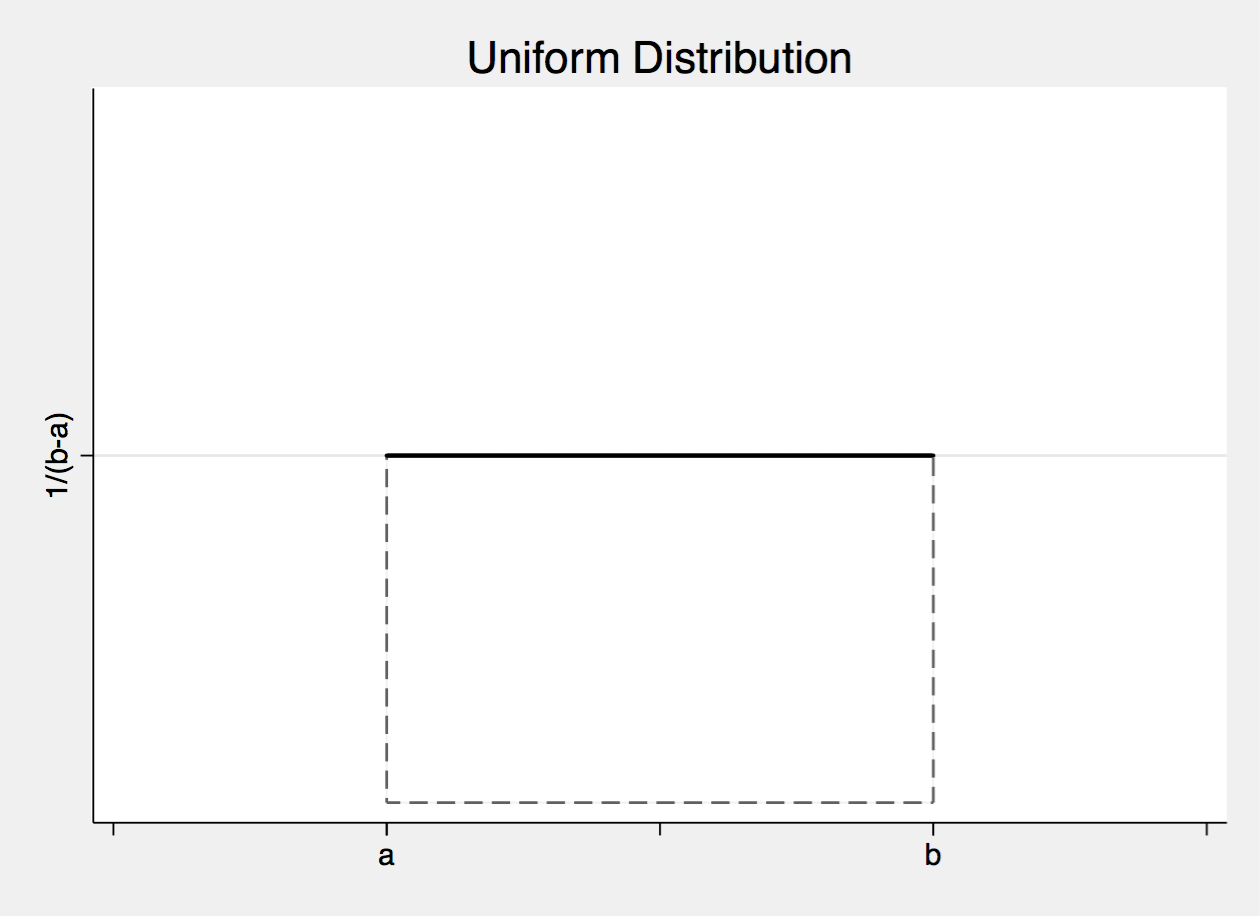
\includegraphics[width=\textwidth]{uniformab.png}}
		\end{column}
		\begin{column}{0.4\textwidth}{
				\begin{enumerate}[label=(\alph*)]
					\item $\frac{b-a}{2}$
					\item $\frac{b+a}{2}$
					\item $\frac{1}{b-a}$
					\item $1$
				\end{enumerate}}
		\end{column}
	\end{columns}
\end{frame}

%\begin{frame}{Midterm Example}
%Consider the probability distribution for random variable X:
%$$f(x)=.08x, 0\leq x \leq 5$$
%Find $E[X]$
%\end{frame}






\begin{frame}{Properties of Expectation}
	A trick that will make our lives easier is that expectations are a \alert{linear operator} which means you can move the sum outside of the $E$ function. 
	
	Let X, Y be random variables and a, b be constants. Then:
	\begin{itemize}
		\item E(a)=a
		\item E(aX) = aE(X)
		\item E(X + b) = E(X) + b
		\item E(aX+b) = aE(X) + b
		\item E(X + Y) = E(X) + E(Y)
	\end{itemize}
\end{frame}

\begin{frame}{Clicker Question}
	Suppose that the expected income in Boulder is \$90,000 and the tax rate is 10\%. Then the post-tax income is Y=0.9X where X is annual income of a Boulder resident. What is the expected post-tax income for a Boulder resident, E(Y)?
	
	\begin{enumerate}[label=(\alph*)]
		\item \$8,000
		\item \$90,000
		\item \$9,000
		\item \$81,000
	\end{enumerate}
\end{frame}

%\begin{frame}{Independence of Expectations}
%Often we will be interested in the expectation of the product of two random variables, X and Y. In general:
%$$E(XY)=\sum_{x\in S_x} \sum_{y\in S_y} x \cdot y \cdot P(x \cap y)$$
%Howver, if X and Y are independent, it's easy to show that E(XY)=E(X)E(Y). 
%\begin{itemize}
%\item This simple formula will come in handy when we discuss covariance
%\end{itemize}
%\end{frame}

\begin{frame}{Definition of Variance}
	Recall the variance of a sample is $s^2 = \frac{1}{n-1} \sum_{i=1}^n (X_i - \bar{X})^2$

	We can use expectations to define a similar expression for the population variance. 
	
	Let X be a random variable with $E(X)< \infty$. Then the \alert{variance} of X is:
	\[ 
		var(X) = E[(X-E(X))^2] 
	\]

	Imagine writing this out as an integral and solving it. Would not be fun. \textbf{Instead, we will be using a much simpler equation to calculate variance...}
\end{frame}

\begin{frame}{Alternate Form}
	Note that we can write,
	\begin{align*}
		Var(X) & = E[ \left(X - E(X) \right)^2 ] = E[ X^2 - 2X\cdot E(X) + [E(X)]^2 ] \\
		       & = E(X^2) - 2E(X)\cdot E(X) + [E(X)]^2                                \\
		       & = E(X^2) - 2[E(X)]^2 + [E(X)]^2                                      \\
		       & = E(X^2) - [E(X)]^2,                                                 
	\end{align*}
	
	$Var(X)=E(X^2)-[E(X)]^2$ is a much simpler expression of variance (and the one you should use)
\end{frame}

\begin{frame}{Properties of Expectation}
	We can compose E with a function of a random variable, g(X).
	
	\[ 
		E[g(X)]= \sum_{x\in S} g(x) \cdot p_x(x)
	\] 

	The result is the expected value of g(X). We will use this property to calculate $E[X^2]$
\end{frame}

\begin{frame}{Example}
	Let $g(X) = X^2$. What is E[g(X)]?

	\begin{align*}
		E[g(X)] = \sum x^2\cdot p_X(x) &   
	\end{align*}
		
	While $E(X)$ is called the \alert{first moment}, we call $E(X^2)$ the \alert{second moment} of X. 
		
	Therefore, we calculate $E[X^2]$ using the following equation: 
		
	\[ E[X^2] = \sum x^2*p(x) \]
\end{frame}


\begin{frame}{Example}
	Let X be the number of heads in two coin flips. 

	\[ 
		E(X) = 0 \cdot (\frac{1}{4})+ 1 \cdot (\frac{1}{2}) + 2 \cdot (\frac{1}{4}) = \frac{1}{2} + \frac{1}{2} = 1
	\]
	\[ 
		E(X^2) = 0^2 \cdot (\frac{1}{4})+ 1^2 \cdot (\frac{1}{2}) + 2^2 \cdot  (\frac{1}{4}) = \frac{1}{2} + 1 = \frac{3}{2}
	\]
		
	This means that $V(X)=E(X^2)-[E(X)]^2 = \frac{3}{2}-1^2 = \frac{1}{2}$
		
	\textbf{Never square probabilities when solving $E(X^2)$. Only square $X$ values}
\end{frame}

\begin{frame}{Properties of Variance}
	There are several important properties of the variance operator:
	\begin{itemize}
		\item $Var(a)=0$
		\item $Var(aX)=a^2Var(X)$
		\item $Var(aX+b) = a^2Var(X)$
		\item $Var(aX+bY)=a^2Var(X)+b^2Var(Y)+2ab\cdot cov(X,Y).$\footnote{we will discuss more about covariance later, when X and Y are independent then the covariance is zero}
	\end{itemize}
\end{frame}

\begin{frame}{Clicker Question}
	Recall that in Boulder the mean income is \$90,000 and the tax rate is 10\%. Suppose that the variance of income in Boulder is \$1,000. What is the variance of post-tax income, Y=0.9X?
	\begin{enumerate}[label=(\alph*)]
		\item \$900
		\item \$1000
		\item \$810
		\item \$800
	\end{enumerate}
\end{frame}

\begin{frame}{Calculating Variance}
	The equation we use for variance is $V[X]=E[X^2]-(E[X])^2$.

	When X is \alert{discrete}:
	\[
		\sum_x x^2*p(x) -(\sum_x x*p(x))^2
	\]
	When X is \alert{continuous}:
	\[
		\int^\infty_{-\infty} x^2 * f(x) \ dx - \left(\int^\infty_{-\infty} x * f(x) \ dx \right )^2
	\]
\end{frame}

\begin{frame}{Midterm Example}
	Consider the probability distribution for random variable Y;
	\[
		f(x)=.08x, 0\leq x \leq 5
	\]
	Find $V[X]$:
	\[
		V[X]=\int_{-\infty}^\infty x^2 * f(x) \ dx - \left[ \int_{-\infty}^\infty x * f(x) \ dx \right]^2
	\]
	\[
		= \int_0^5 x^2 * .08x \ dx \left[\int_0^5 x * .08x \ dx \right]^2= \int_0^5 .08x^3 \ dx - \left[  \int_0^5 .08x^2 \ dx \right]^2
	\]

	\[
		=\frac{.08x^4}{4} \Big|_0^5 - \left( \frac{.08x^3}{3}  \Big|_0^5\right) ^2= 12.5-(3.3)^2=1.61 
	\]
\end{frame}


%\begin{frame}{Midterm Example}
%
%Consider the probability distribution for random variable X:
%\begin{center}
%\begin{tabular}{|c|c|c|c|c|}
%\hline
%X & 1 & 2 & 3 & 5 \\
%P(X) & 0.1 & 0.2 & 0.2 & p \\
%\hline
%\end{tabular}
%\end{center}
%\begin{enumerate}[label=(\alph*)]
%\item What must the value of $p$ be such that this is a valid probability distribution?
%\item Find the expectation of X
%\item Find the variance of X
%\end{enumerate}
%
%\end{frame}

\begin{frame}{Midterm Example}
	Consider the probability distribution for random variable X:
	
	\begin{center}
		\begin{tabular}{|c|c|c|c|c|}
			\hline
			X    & 2    & 4    & 6    & 8   \\ \hline
			P(X) & 0.19 & 0.07 & 0.35 & $p$ \\
			\hline
		\end{tabular}
	\end{center}
	\begin{enumerate}[label=(\alph*)]
		\footnotesize{\item Find the expectation of X
			\item  Find the variance of X
			\item A friend says, the expected value of X is 5. To justify this he says, ``Well X could be 2,4,6, or 8, so the average is $\frac{2+4+6+8}{4} = 5$". Why is your friend wrong? Why isn't $E[X]=5?$ (1-2) sentences. 
			\item Let $Y\sim N(4,1)$. Random variable W is defined as W=2X+3Y. Given your information about the random variables X and Y. What is E[W]? What is V[W]? (assuming X \& Y are independent) }
	\end{enumerate}
\end{frame}

\begin{frame}

	

\end{frame}

\begin{frame}{Midterm Example}
	Consider the probability distribution for random variable Y:
	$$f(y)= 8y, 0\leq y \leq \frac{1}{2}$$
	\begin{enumerate}[label=(\alph*)]
		\item Find $E[Y]$
		\item Find $P(Y<\frac{1}{3})$
		\item Find $P(Y=\frac{1}{4})$
		\item Find $V[Y]$
		\item Find $P(\frac{3}{4}<Y<1)$
	\end{enumerate}
\end{frame}

\begin{frame}

	

\end{frame}


\end{document}